\documentclass{scrartcl}
\usepackage[utf8]{inputenc}
\usepackage[T1]{fontenc}
\usepackage[a4paper]{geometry}
\usepackage{graphicx}
\usepackage{hyperref}
\usepackage{float}
\usepackage{mathtools}
\usepackage{textcomp}
\usepackage{gensymb}
\usepackage[ngerman]{babel}
\usepackage{epstopdf}
\usepackage{titlesec}
\renewcommand{\arraystretch}{1.3}
\setcounter{secnumdepth}{5}
\setcounter{tocdepth}{5}
\makeatletter
\renewcommand\paragraph{\@startsection{paragraph}{4}{\z@}%
  {-3.25ex\@plus -1ex \@minus -.2ex}%
  {1.5ex \@plus .2ex}%
  {\normalfont\normalsize\bfseries}}
\newcommand*{\tline}{%
  \ifmeasuring@
  % first measuring run
  \else
  % second run
  % \typeout{\meaning\maxcolumn@widths}% debug info
  \ifodd\column@
  \expandafter\rlap
  \else
  \expandafter\llap
  \fi
     {%
       \vrule height-1ex depth \dimexpr1ex+.4pt\relax width
       \ifcase\numexpr\column@+1\expandafter\relax
       \maxcolumn@widths
       \fi
     }%
     \fi
}
\makeatother
\restylefloat{table}
\newcommand{\mytitle}{Übung 5)}
\hypersetup{
  colorlinks=true,
  linkcolor=blue,
  pdftitle=\mytitle,
  pdfauthor={Stefan Hermeter},
}
\begin{document}
\title{\mytitle:Uebungspacket 5}
\subtitle{CreateFile, AnalyzeText, DynamicText}
\date{\today}
\author{Stefan Hermeter \texttt{\href{mailto:stefan.hermeter@gmx.at}{stefan.hermeter@gmx.at}}\\
  Klasse: 5ABETi\\
  Schuljahr: 2015/16}
\pagenumbering{gobble}
\maketitle
\pagenumbering{roman}
\newpage
\tableofcontents
\listoffigures
\newpage
\pagenumbering{arabic}
\section{Aufgabenstellung}
In dieser Uebung sind 3 Programme zu erstellen.(CreatFile, AnalyzeText, DynamicText)
\subsection{CreateFile}
Schreiben Sie ein Programm CreateFile welches einen Text, bestehend aus mehreren Zeilen in einer Datei speichert. Lesen Sie dazu Strings ueber die Standardeingabe (Tastatur) ein und schreiben Sie die Strings mit einer
Zeilennummer versehen in eine Datei. Die Datei soll den Namen 'uebtext.txt' erhalten. Speichern Sie die Datei in einem entsprechenden Pfad, z.B: C://SEN/Uebungspaket. Lesen Sie von der Datei die einzelnen Zeilen ein und geben Sie diese zur Kontrolle auf die Standardausgabe aus. Kontrollieren Sie zusätzlich mit einem Editor die gespeicherten Daten in der Datei. Wird die option '-a' für append angegeben, so oeffnen Sie die Datei im Append-Modus, sodass die Zeilen angehaengt werden. (Die Zeilennummern beginnen wieder bei 01)
\subsection{AnalyzeText}
Schreiben Sie ein Programm AnalyzeText, welches die Datei aus Uebung 1 zeichenweise einliest. Suchen Sie nach einem XML-Tag und geben Sie den Elementnamen und den Inhalt auf die Standardausgabe aus.

Bei ungueltigen XML-Elementen, geben Sie fuer die betreffende Zeile, eine Fehlermeldung "kein oder ungueltiges XML-Element" aus. Achten Sie auf die Abfrage des Dateiendes, z.B. mit der Funktion feof() oder EOF! Hinweis: es gilt die Einschraenkung, dass sich ein XML-Element nur in einer Zeile befinden darf.
\subsection{DynamicText}
Schreiben Sie ein Programm DynamicText, welches die Zeilen einer Datei (z.B. aus Uebung 1) in den Speicher einliest. Die Zeilen sollen als String-Array gespeichert und das String-Array dynamisch verwaltet werden. Verwenden Sie dazu die Funktionen malloc() und realloc(). Dadurch ist es moeglich eine Datei in den Speicher zu laden, ohne vorher zu wissen wie grosz diese Datei ist. Geben Sie die Anzahl der gelesenen Zeilen als Information aus. Der Benutzer soll nun durch Eingabe waehlen koennen welche Zeile er sehen moechte. Geben Sie die Zeile entsprechend der eingegebenen Zeilennummer, inklusive 2 Zeilen vorher und 2 Zeilen nachher auf die Standardausgabe aus. Die gesuchte Zeile soll mit einer anderen Farbe markiert werden. Eine Eingabe von 0 beendet das Programm. Beachten Sie vor dem Beenden des Programmes, dass der dynamische Speicher wieder frei gegeben werden muss.
\section{./CreateFile}
\subsection{Programmablaufplan}
\begin{figure}[H]
  \centering
  \includegraphics[width=0.9\linewidth]{images/CreateFile.eps}
  \caption{Programmablauf-CreateFile}
  \label{fig:digraph}
\end{figure}
\subsection{Resourcen Aufteilung}
\subsubsection{C-File}
\begin{itemize}
\item CreateFile.c
\end{itemize}
\subsubsection{Verwendetet Libaries}
\begin{itemize}
\item stdlib.h
\item stdio.h
\item unistd.h
\item ctype.h
\item string.h
\end{itemize}
\subsection{Test}
\subsubsection{./CreateFile}
\begin{figure}[H]
  \centering
  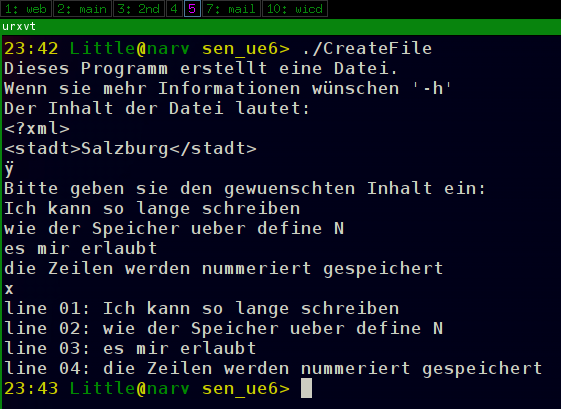
\includegraphics[width=0.9\linewidth]{images/Test_CreateFile.png}
  \caption{./CreateFile}
  \label{fig:digraph}
\end{figure}
\subsubsection{./CreateFile -h und ./CreateFile -a}
\begin{figure}[H]
  \centering
  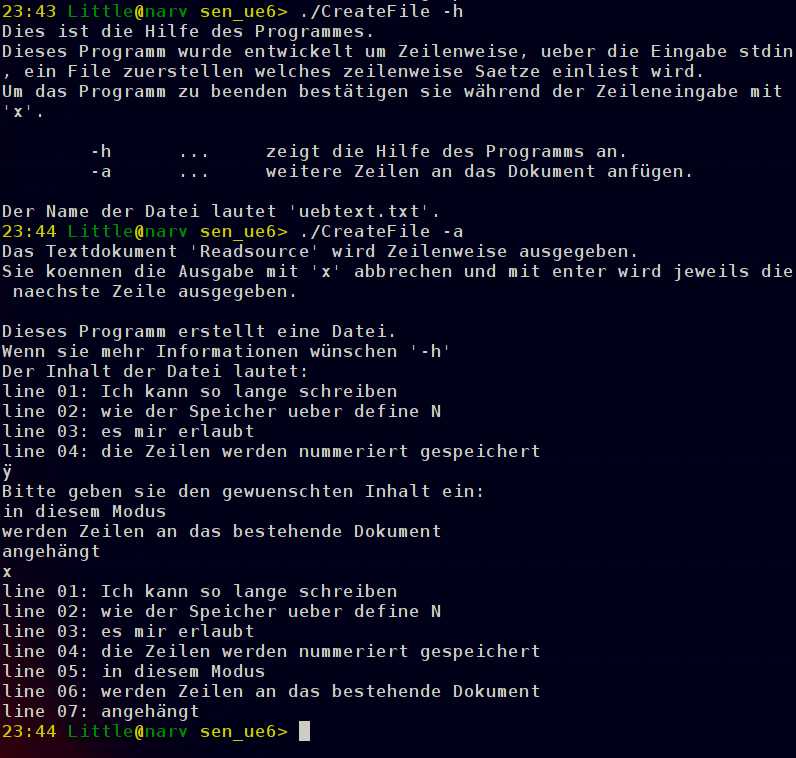
\includegraphics[width=0.9\linewidth]{images/Test_CreatFile_a.png}
  \caption{./CreateFile -h und ./CreateFile -a}
  \label{fig:digraph}
\end{figure}
\subsection{Ablauf ./CreateFile}
Das Programm hat zwei Argumente mit den es gestartet werden kann. (-a oder -h) Die dritte Option wäre das Programm ohne Argument zustarten.
./CreateFile:
Es wird zuerst überprüft ob eine Datei mit dem Namen 'uebtext.txt' existiert. Tritt dieser Fall ein wird der Inhalt der Datei auf dem Bildschirm wiedergegeben. Der Inhalt wird allerdings geloescht. Man kann jetzt x-beliebige Zeilen in die Datei schreiben. Mit x wird das Programm beendet.
./CreateFile -h:
Mit dem Argumenten aufruf '-h' wird lediglich die Hilfe des Programms ausgegeben.
./CreateFile -a:
Mit dem Argument -a wird wie oben ohne Argument ueberprueft ob diese Datei vorhanden ist. Wenn sie nicht vorhanden ist wird diese Datei erstellt. Der Inhalt falls vorhanden bleibt bestehen und x Zeilen koennen angefuegt werden. Mit x wird das Programm wieder beendet.
\section{./AnalyzeText}
\subsection{Programmablaufplan}
\begin{figure}[H]
  \centering
  \includegraphics[width=0.9\linewidth]{images/AnalyzeText.eps}
  \caption{Programmablauf-AnalyzeText}
  \label{fig:digraph}
\end{figure}
\subsection{Resourcen Aufteilung}
\subsubsection{C-File}
\begin{itemize}
\item AnalyzeText.c
\end{itemize}
\subsubsection{Verwendetet Libaries}
\begin{itemize}
\item stdlib.h
\item stdio.h
\item unistd.h
\item ctype.h
\item string.h
\end{itemize}
\subsection{Test}
\begin{figure}[H]
  \centering
  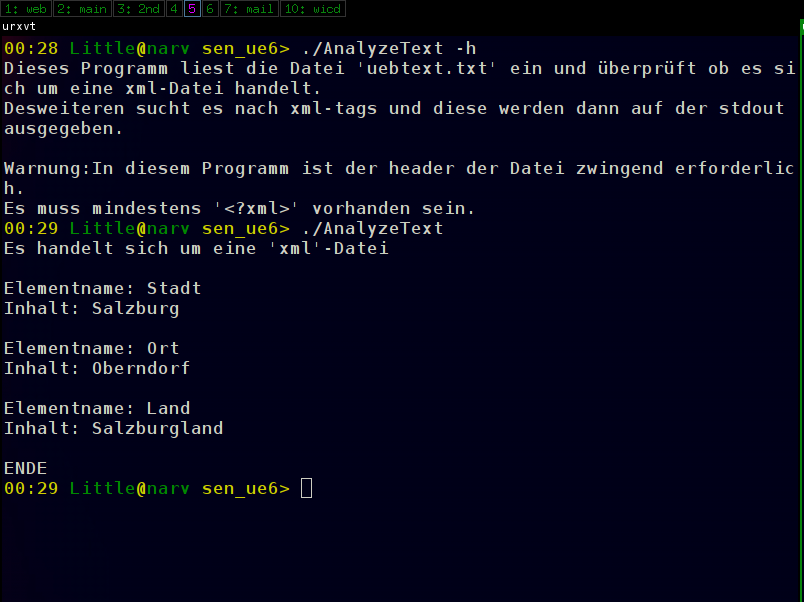
\includegraphics[width=0.9\linewidth]{images/Test_AnalyzeText.png}
  \caption{./AnalyzeText und ./AnalyzeText -h}
  \label{fig:digraph}
\end{figure}
\subsection{Ablauf ./AnalyzeText}
Das Programm kontrolliert zuerst die Argumenteneingabe, wurde hier ein falsches Argument eingegeben, gibt er dies auf der Kommandozeile aus und schreibt ausserdem einen Hinweis zur Hilfe des Programms.
Wurde kein Argument eingegeben oeffnet das Programm die Datei 'uebtext.txt' und liest das Programm in den Speicher ein. Über die Funktion xml\_finder wird dann ueberprueft ob es sich um eine xml-Datei handelt.
WICHTIG:In diesem Programm ist in der 1ten Zeile ein Header erforderlich '<?xml>'!
Handelt sich um jene Datei wir ueber die Funktion xml\_tag die Datei wie gewuenscht ausgegeben.
\section{./DynamicText}
\subsection{Programmablaufplan}
\begin{figure}[H]
  \centering
  \includegraphics[width=0.9\linewidth]{images/DynamicText.eps}
  \caption{./AnalyzeText und ./AnalyzeText -h}
  \label{fig:digraph}
\end{figure}
\subsection{Resourcen Aufteilung}
\subsubsection{C-File}
\begin{itemize}
\item DynamicText3.c
\end{itemize}
\subsubsection{Verwendetet Libaries}
\begin{itemize}
\item stdlib.h
\item stdio.h
\item unistd.h
\item ctype.h
\item string.h
\end{itemize}
\subsection{Test}
\begin{figure}[H]
  \centering
  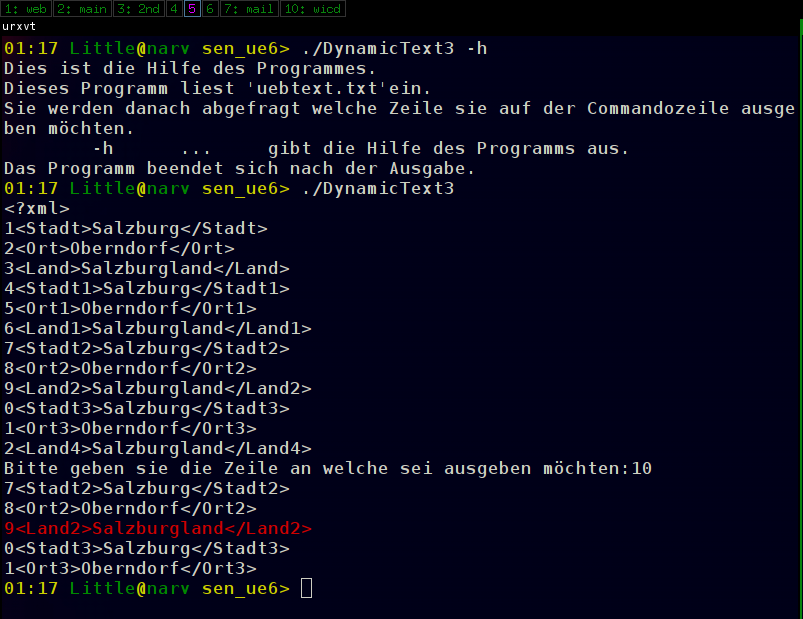
\includegraphics[width=0.9\linewidth]{images/Test_DynamicText.png}
  \caption{./AnalyzeText und ./AnalyzeText -h}
  \label{fig:digraph}
\end{figure}
\subsection{Ablauf ./DynamicText3}
Wird das Programm wird mit dem Argument '-h' geoeffnet so wird die Hilfe ausgegeben und das Programm beendet. Wird ein falsches Argument eingegeben so wird auf die Hilfe aufmerksam gemacht und das Programm wird beendet. Lauft das Programm standard gemaesz durch so wird in einer while schleife mit dem fgets zeilenweise die Datei 'uebtext' eingelesen und der Speicher dynamisch Zeile für Zeile hinzugefügt. Danach wird abgefragt welche Zeile ausgegeben werden soll, ist die Eingabe kleiner gleich 2 oder mehr als die vorhanden Zeilen. So wird über eine Ausgabe aufmerksam gemacht das dies nicht moeglich ist und nochmals abgefragt.

Hinweis: Dieses Programm wurde mit 888 Zeilen getestet und es trat kein Fehler auf.
\end{document}
